\scanpage{35}\mspage{5}

allusion, one should be able to 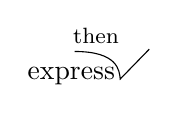
\begin{tikzpicture}[baseline=(alorsb.base)]
\node[anchor=base west,inner sep=0pt] (alorsb) at (0,0) {express};
\node[anchor=south east,inner sep=0pt,font=\footnotesize] at ([xshift=.05cm,yshift=.30cm]alorsb.north east) {\inserted{then}};
\draw ([xshift=-.52cm,yshift=.20cm]alorsb.north east) .. controls ([xshift=.03cm,yshift=.20cm]alorsb.north east) and ([xshift=.05cm,yshift=-.04cm]alorsb.north east) .. ([xshift=.06cm,yshift=-.15cm]alorsb.north east) -- ([xshift=.43cm,yshift=.23cm]alorsb.north east);
\end{tikzpicture}
the \uline{homotopy type} \uline{of} $\deleted{\unsure{Z}}X$ (and not only its $\Pi_1$) in terms of the 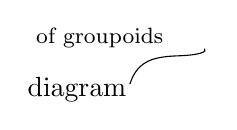
\begin{tikzpicture}[baseline=(groupb.base)]
\node[anchor=base west,inner sep=0pt] (groupb) at (0,0) {diagram};
\node[anchor=south east,inner sep=0pt,font=\footnotesize] at ([xshift=.47cm,yshift=.36cm]groupb.north east) {\inserted{of groupoids}};
\draw ([xshift=.04cm,yshift=-.10cm]groupb.north east) .. controls ([xshift=.14cm,yshift=.22cm]groupb.north east) and ([xshift=.38cm,yshift=.25cm]groupb.north east) .. ([xshift=.67cm,yshift=.26cm]groupb.north east) .. controls ([xshift=.92cm,yshift=.27cm]groupb.north east) and ([xshift=1.03cm,yshift=.31cm]groupb.north east) .. ([xshift=.99cm,yshift=.35cm]groupb.north east);
\end{tikzpicture} (8), or what amounts to the same, of the diagram of groups (10).

In any case, it is clear (independent-
ly of any hypothesis of vanishing of certain $\Pi_i$, or of local normal triviality) how to reconstruct, in terms of diagram 8, the 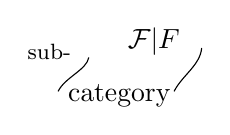
\begin{tikzpicture}[baseline=(catone.base)]
\node[anchor=base west,inner sep=0pt] (catone) at (0,0) {category};
\node[anchor=south east,inner sep=0pt,font=\footnotesize] at ([xshift=.05cm,yshift=.30cm]catone.north west) {\inserted{\unsure{sub-}}};
\node[anchor=south east,inner sep=0pt] at ([xshift=.12cm,yshift=.35cm]catone.north east) {\inserted{$\unsure{\mathcal F|\mathfrak F}$}};
\draw ([xshift=-.12cm,yshift=-.10cm]catone.north west) .. controls ([xshift=-.03cm,yshift=.08cm]catone.north west) and ([xshift=.24cm,yshift=.17cm]catone.north west) .. ([xshift=.27cm,yshift=.33cm]catone.north west);
\draw ([xshift=.04cm,yshift=-.10cm]catone.north east) .. controls ([xshift=.14cm,yshift=.10cm]catone.north east) and ([xshift=.37cm,yshift=.23cm]catone.north east) .. ([xshift=.39cm,yshift=.45cm]catone.north east);
\end{tikzpicture} in the category of sheaves on $X$, \deleted{of which} formed of the $F$ such that one has

\[
(16)\qquad F\mid X^*\quad\text{and}\quad F\mid Y\quad\text{locally trivial}\unsure{,|;}
\]

This 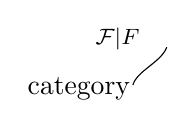
\begin{tikzpicture}[baseline=(cattwob.base)]
\node[anchor=base west,inner sep=0pt] (cattwob) at (0,0) {category};
\node[anchor=south east,inner sep=0pt,font=\footnotesize] at ([xshift=.12cm,yshift=.34cm]cattwob.north east) {\inserted{$\unsure{\mathcal F|\mathfrak F}$}};
\draw ([xshift=.03cm,yshift=-.10cm]cattwob.north east) .. controls ([xshift=.08cm,yshift=.08cm]cattwob.north east) and ([xshift=.39cm,yshift=.19cm]cattwob.north east) .. ([xshift=.46cm,yshift=.38cm]cattwob.north east);
\end{tikzpicture} is indeed equivalent to that of systems

\[
(17)\qquad (E_{X^*},E_{Y,X}\mathpunct{\begin{tikzpicture}[baseline=-.25ex]
\node[inner sep=0pt] at (.03,.23) {$\cdot$};
\node[inner sep=0pt] at (0,.12) {$\cdot$};
\node[inner sep=0pt] at (.11,-.03) {$,$};
\end{tikzpicture}}\varphi)
\]

\deleted{\unsure{formed}} 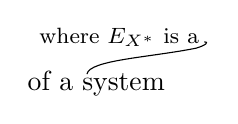
\begin{tikzpicture}[baseline=(rewriteb.base)]
\node[anchor=base west,inner sep=0pt] (rewriteb) at (0,0) {\deleted{\unsure{of a}} system};
\node[anchor=south west,inner sep=0pt,font=\footnotesize] at ([xshift=.15cm,yshift=.30cm]rewriteb.north west) {\inserted{where $E_{X^*}$ is a}};
\draw ([xshift=.76cm,yshift=-.04cm]rewriteb.north west) .. controls ([xshift=.79cm,yshift=.14cm]rewriteb.north west) and ([xshift=1.55cm,yshift=.17cm]rewriteb.north west) .. ([xshift=2.15cm,yshift=.29cm]rewriteb.north west) .. controls ([xshift=2.28cm,yshift=.33cm]rewriteb.north west) and ([xshift=2.31cm,yshift=.37cm]rewriteb.north west) .. ([xshift=2.25cm,yshift=.37cm]rewriteb.north west);
\end{tikzpicture} local on \begin{tikzpicture}[baseline=(coverb.base)]
\node[anchor=base west,inner sep=0pt] (coverb) at (0,0) {$\Pi_1X^*$};
\node[anchor=south west,inner sep=0pt,font=\footnotesize] (covera) at ([xshift=-.2cm,yshift=.58cm]coverb.north east) {\inserted{($\unsure{\leftrightarrow|\Leftrightarrow}$ a covering \begin{tikzpicture}[baseline=(etaddb.base)]
\node[anchor=base west,inner sep=0pt] (etaddb) at (0,0) {of $X^{\unsure{*|+}}$};
\node[anchor=south east,inner sep=0pt,font=\footnotesize] at ([xshift=.12cm,yshift=.34cm]etaddb.north west) {\inserted{\unsure{étale|étale}}};
\draw ([xshift=.03cm,yshift=-.10cm]etaddb.north west) .. controls ([xshift=.08cm,yshift=.08cm]etaddb.north west) and ([xshift=.39cm,yshift=.19cm]etaddb.north west) .. ([xshift=.46cm,yshift=.38cm]etaddb.north west);
\end{tikzpicture})}};
\draw ([xshift=.05cm,yshift=-.03cm]coverb.north east) .. controls ([xshift=.08cm,yshift=.36cm]coverb.north east) and ([xshift=.20cm,yshift=-.10cm]covera.south west) .. ([xshift=.65cm,yshift=-.10cm]covera.south west) -- ([xshift=1.45cm,yshift=-.10cm]covera.south west);
\draw ([xshift=1.49cm,yshift=-.10cm]covera.south west) -- ([xshift=.08cm,yshift=-.04cm]covera.south east) .. controls ([xshift=.28cm,yshift=-.01cm]covera.south east) and ([xshift=.20cm,yshift=.10cm]covera.south east) .. ([xshift=.14cm,yshift=.09cm]covera.south east);
\end{tikzpicture}, $E_{Y,X}$ a local system on \begin{tikzpicture}[baseline=(piaddb.base)]
\node[anchor=base west,inner sep=0pt] (piaddb) at (0,0) {$\Pi_1\mathcal V_{Y,X}$};
\node[anchor=south west,inner sep=0pt,font=\footnotesize] at ([xshift=-.10cm,yshift=.32cm]piaddb.north east) {\inserted{$\xleftarrow{\approx}\Pi_1Y$}};
\draw ([xshift=.06cm,yshift=-.13cm]piaddb.north east) .. controls ([xshift=-.03cm,yshift=.13cm]piaddb.north east) and ([xshift=.35cm,yshift=.20cm]piaddb.north east) .. ([xshift=.98cm,yshift=.42cm]piaddb.north east);
\end{tikzpicture} ($\leftrightarrow$ an étale covering of $Y$) and $\varphi$ a homomorphism of local systems on $\Pi_1\mathcal V^*_{Y,\unsure{\lambda|X}}$

\margin{34}
